%# -*- coding: utf-8 -*-
\chapter{效用}
\label{chp:utility}

\section{无差异曲线和效用函数}%Indifference curve

\section{效用函数的单调变换}%Indifference curve
与基数效用论不同,基于偏好分析的序数效用论并不要求效用函数具备“准确”的数值,从这个角度来看某种偏好的效用函数表达的是“序数指数”——当然,这只是我自娱自乐的文字游戏。

假设偏好对应的效用函数为$u=v(x,y)$,当$u_1>u_2$,意味着$f(u_1)>f(u_2)$时,则称$f(v)$为原效用函数$u(x)$的单调变换。

这意味着在经济意义满足的条件下只要函数$f(\cdot)$为单调函数,就可以将既有的效用函数$u=u(x,y)$变换为$u=f[v(x,y)]$而不违背该效用函数背后的偏好特征,也不改变无差异曲线的特征。

常见的单调变换有:
\begin{compactitem}
\item 乘上一个整数:$u=av$,其中$a>0$;
\item 加上任意常数:$u=v+a$,其中$a$为常数;
\item 取奇数次幂:$u=v^k$,其中$k$为奇数;
\item 取对数(指数)函数:$u=\ln v$,或$u=e^v$;
\end{compactitem}

\section{边际效用}
若保持其他商品消费数量不变,第$i$种商品数量变动1单位所带来的总效用变化称为该商品(在该消费数量上的)边际效用,对应的函数称为边际效用函数。

假设效用函数为$u=u(x_1,x_2,\cdots,x_n)$,则第$i$种商品的边际效用函数为
\begin{equation}
MU_i=\frac{\partial u(\cdot)}{\partial x_i}
\label{eq:marginal-utility-function}
\end{equation}

在序数论中边际效用的数值是无关紧要的,因为效用函数的出的总效用本身就是无关紧要的。例如$u=x^2y^2$的边际效用函数为$u_x=2xy^2$,在$y$一定的情况下$u_x$在数值上显然是递增的。在序数论中为消费者最优提供参考依据的是商品之间的关系——边际替代率。

\section{边际替代率}
\label{sec:marginal-rate-of-substitution}
\index{marginal 边际!marginal rate of substitution}
假设效用函数为$u=u(x_1,x_2,\cdots, x_n)$,若增加第$i$中商品的消费数量且保持效用水平不变,第$j$种商品消费数量作何调整?
\begin{equation}
du = \frac{{\partial u(\cdot)}}{{\partial {x_1}}}d{x_1} + \frac{{\partial u(\cdot)}}{{\partial {x_2}}}d{x_2} +  \cdots  + \frac{{\partial u(\cdot)}}{{\partial {x_i}}}d{x_i} +  \cdots  + \frac{{\partial u(\cdot)}}{{\partial {x_j}}}d{x_j} +  \cdots + \frac{{\partial u(\cdot)}}{{\partial {x_n}}}d{x_n}
\end{equation}
为保持总效用不变,取$du=0$;只变动第$i$、$j$两种商品,则$dx_k=0$,其中$k=1,2,\cdots,n ~ k \ne i,j$,得到
\begin{equation}
\frac{{\partial u(\cdot)}}{{\partial {x_i}}}d{x_i} + \frac{{\partial u(\cdot)}}{{\partial {x_j}}}d{x_j} = 0
\end{equation}
边际偏好替代率为
\begin{equation}
%\begin{split}
MRS_{{i}~\text{for}~{j}} = \frac{{d{x_j}}}{{d{x_i}}} =  - \left. {\frac{{\partial u(\cdot)}}{{\partial {x_i}}}} \middle/ {\frac{{\partial u(\cdot)}}{{\partial {x_j}}}} \right. = -\frac{MU_i}{MU_j}
\label{eq:marginal-rate-of-substitution}
%\end{split}
\end{equation}

前文提到效用函数的单调变换不改变偏好特征,包括不改变商品之间的边际替代率。对效用函数做单调变换
\begin{equation}
u = u(\cdot)\mathop  {\xrightarrow{\text{单调变换}}} u = f[u(\cdot)]
\label{eq:xiaoyong-dandiaobianhuan}
\end{equation}
根据复合函数求导的链式法则
\begin{equation}
%\begin{split}
MRS_{{i}~\text{for}~{j}} = \frac{{d{x_j}}}{{d{x_i}}}	=  - \left. {f'[u(\cdot)]\frac{{\partial u(\cdot)}}{{\partial {x_i}}}} \middle/ {f'[u(\cdot)]\frac{{\partial u(\cdot)}}{{\partial {x_j}}}} \right. = -\frac{MU_i}{MU_j}
\label{eq:marginal-rate-of-substitution-monly}
%\end{split}
\end{equation}

\section{常见的偏好类型与其效用函数}

\subsection[线性]{线性效用函数}
\index{utility function 效用函数!linear 线性}
\index{preference 偏好!linear 线性偏好}
\index{preference 偏好!perfect substitutes 完全替代品}
\index{functions 函数!linear function 线性函数}

如图(\ref{fig:indefferent-curves_linear-function}),线性效用函数形如$u=f(x,y)=\alpha x + \beta y$,则商品$X$、$Y$的边际效用函数分别为,
\[
MU_X = f_1=\alpha \text{,} MU_Y = f_2=\beta
\]
无差异曲线的斜率以及边际替代率分别为:
\[
\frac{dy}{dx}=-\frac{\alpha}{\beta} \text{,} MRS_{XY} = \frac{\alpha}{\beta}
\]

\begin{figure}[!h]
\colorbox{black!3}{\parbox{\linewidth-2\fboxsep}{%
\centering
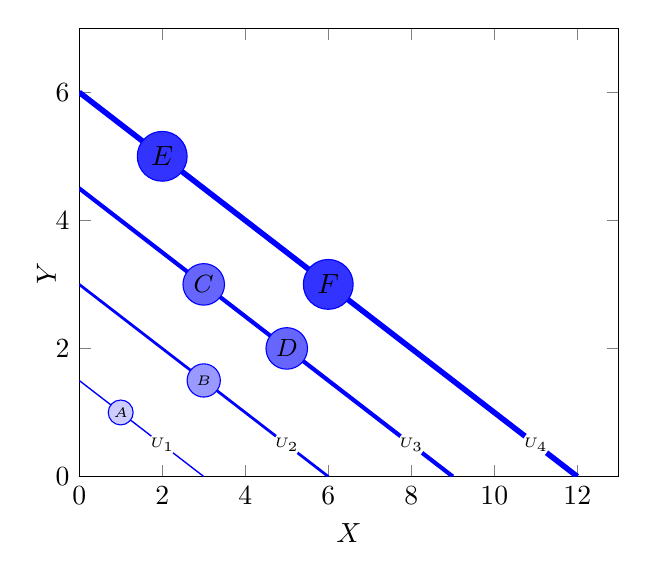
\begin{tikzpicture}
\begin{axis}[
	xmin=0,xmax=13,ymin=0,ymax=7,
	xlabel style={below},xlabel=$X$,ylabel style={left},ylabel=$Y$,
	domain=0:13]
\foreach \utiliy in {3.0,6.0,9.0,12.0}
{\edef\temp{\noexpand
\addplot[draw=blue,line width=\utiliy/6 pt] coordinates {(0,\utiliy/2) (\utiliy,0)};} \temp }
\draw[fill=blue!20,draw=blue,style={font=\tiny}] (axis cs:1,1) circle (4.5pt) node {$A$};
\draw[fill=blue!40,draw=blue,style={font=\tiny}] (axis cs:3,1.5) circle (6pt) node {$B$};
\draw[fill=blue!60,draw=blue,style={font=\small}] (axis cs:3,3) circle (7.5pt) node {$C$};
\draw[fill=blue!60,draw=blue,style={font=\small}] (axis cs:5,2) circle (7.5pt) node {$D$};
\draw[fill=blue!80,draw=blue] (axis cs:2,5) circle (9pt) node {$E$};
\draw[fill=blue!80,draw=blue] (axis cs:6,3) circle (9pt) node {$F$};
\node[fill=white,circle,inner sep=0pt,font=\tiny] at (axis cs:2,0.5) {$U_1$};
\node[fill=white,circle,inner sep=0pt,font=\tiny] at (axis cs:5,0.5) {$U_2$};
\node[fill=white,circle,inner sep=0pt,font=\tiny] at (axis cs:8,0.5) {$U_3$};
\node[fill=white,circle,inner sep=0pt,font=\tiny] at (axis cs:11,0.5) {$U_4$};
%\node[below left] at (axis cs:13,7) {$u = x + 2 y$};
\end{axis}
\end{tikzpicture}%
\caption{线性偏好的无差异曲线}
\label{fig:indefferent-curves_linear-function}
}}
\end{figure}



\subsection[完全互补]{完全互补}\index{preference 偏好!perfect complements 完全互补品}

效用函数为$u=f(x,y) = \min \{\frac{x}{u}, \frac{y}{v}\}$,或$U(x,y) = \min \{ax, by\}$。

\begin{figure}[!h]
\colorbox{black!3}{\parbox{\linewidth-2\fboxsep}{%
\centering
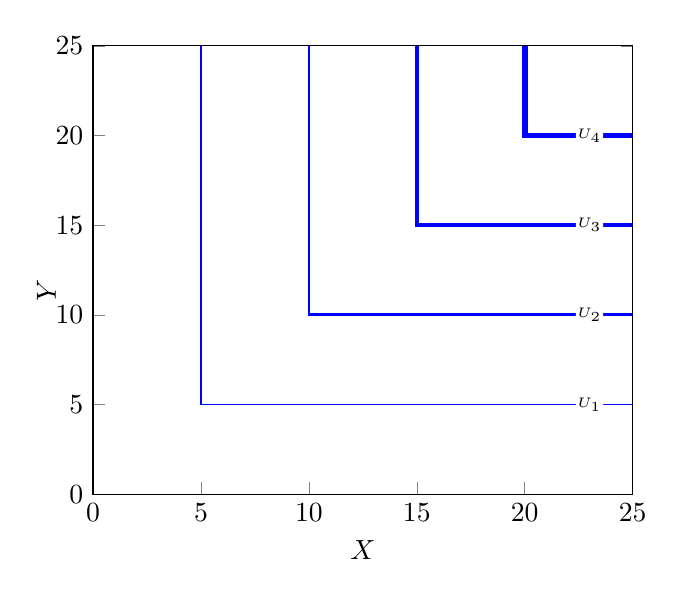
\begin{tikzpicture}
\tikzset{small dot/.style={fill=black,circle,scale=0.3}}
\begin{axis}[
	xmin=0,xmax=25,ymin=0,ymax=25,
	xlabel style={below},xlabel=$X$,
	ylabel style={left},ylabel=$Y$,
	samples=200]
\foreach \utiliy in {5,10,...,20}
{\edef\temp{\noexpand
\addplot[draw=blue,line width=\utiliy/10 pt] coordinates {(\utiliy,25) (\utiliy,\utiliy) (25,\utiliy)};
} \temp }
\node[fill=white,circle,inner sep=0pt,font=\tiny] at (axis cs:23,5) {$U_1$};
\node[fill=white,circle,inner sep=0pt,font=\tiny] at (axis cs:23,10) {$U_2$};
\node[fill=white,circle,inner sep=0pt,font=\tiny] at (axis cs:23,15) {$U_3$};
\node[fill=white,circle,inner sep=0pt,font=\tiny] at (axis cs:23,20) {$U_4$};
\end{axis}
\end{tikzpicture}%
\caption{完全互补型偏好}
\label{fig:wanquanhubu-pianhao}
}}
\end{figure}

\subsection[拟线性]{拟线性偏好}
\label{sec:quasilinear-function}
\index{preference 偏好!quasilinear 拟线性偏好}
\index{functions 函数!quasilinear function 拟线性函数}

\begin{figure}[!h]
\colorbox{black!3}{\parbox{\linewidth-2\fboxsep}{%
\centering
\begin{subfigure}[b]{0.5\textwidth}
\centering
%%%%%%%%%%%%%%%%%%%%%%%%%%%%%%
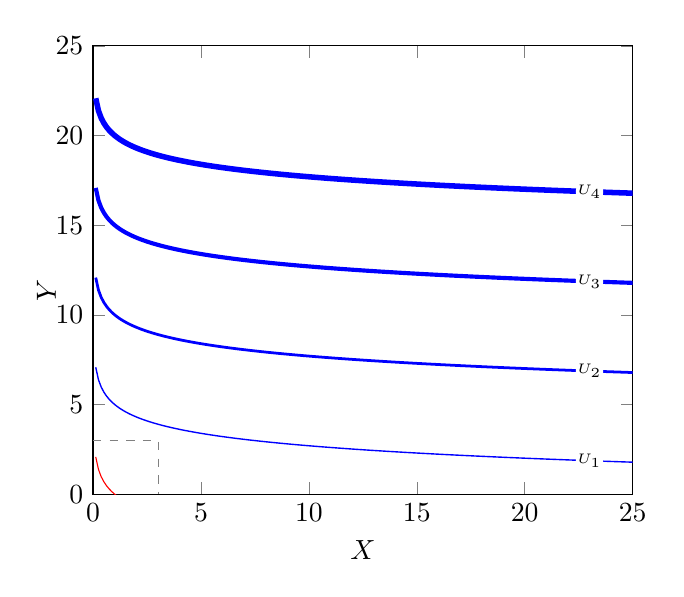
\begin{tikzpicture}
\tikzset{small dot/.style={fill=black,circle,scale=0.3}}
\begin{axis}[
	xmin=0,xmax=25,ymin=0,ymax=25,
	xlabel style={below},xlabel=$X$,
	ylabel style={left},ylabel=$Y$,
	samples=200]
\foreach \utiliy in {5,10,...,20}
{\edef\temp{\noexpand\addplot[draw=blue,domain=0:25,line width=\utiliy/10 pt] {\utiliy-ln(x)};} \temp }
\addplot[draw=red,domain=0:25] {-ln(x)};
\addplot[gray,very thin,dashed] coordinates {(0,3) (3,3) (3,0)};
\node[fill=white,circle,inner sep=0pt,font=\tiny] at (axis cs:23,1.865) {$U_1$};
\node[fill=white,circle,inner sep=0pt,font=\tiny] at (axis cs:23,6.865) {$U_2$};
\node[fill=white,circle,inner sep=0pt,font=\tiny] at (axis cs:23,11.865) {$U_3$};
\node[fill=white,circle,inner sep=0pt,font=\tiny] at (axis cs:23,16.865) {$U_4$};
\end{axis}
\end{tikzpicture}
%%%%%%%%%%%%%%%%%%%%%%%%%%%%%%
\caption[拟线性偏好全图]{全图}
\label{fig:quasilinear-function-all}%
\end{subfigure}%
\begin{subfigure}[b]{0.5\textwidth}
\centering
%%%%%%%%%%%%%%%%%%%%%%%%%%%%%%
\begin{tikzpicture}
\tikzset{small dot/.style={fill=black,circle,scale=0.3}}
\begin{axis}[
	xmin=0,xmax=3,ymin=0,ymax=3,
	xlabel style={below},xlabel=$X$,
	ylabel style={left},ylabel=$Y$,
	samples=200,area style]
\foreach \utiliy in {-3,-2.8,...,3.8}
{\edef\temp{\noexpand\addplot[draw=blueL,domain=0:3,thin] {\utiliy-ln(x)};} \temp }
\addplot[domain=0:3,draw=red,ultra thick] {-ln(x)};
\end{axis}
\end{tikzpicture}
%%%%%%%%%%%%%%%%%%%%%%%%%%%%%%
\caption[拟线性偏好局部图]{局部图}
\label{fig:quasilinear-function-jubu}%
\end{subfigure}
\caption[拟线性偏好的无差异曲线]{拟线性偏好 $U(x,y) = \ln x + y$}
\label{fig:quasilinear-function}%
}}
\end{figure}

如图(\ref{fig:quasilinear-function}),拟线性偏好的效用函数形如$u=f(x,y)=v(x) + y$,整个无差异曲线族可以由其中任何一条曲线沿纵轴平移得到。则商品$X$、$Y$的边际效用函数分别为,
\[
MU_X = f_1 =v'(x) \text{,} MU_Y = f_2 =1
\]
无差异曲线的斜率以及边际替代率分别为:
\[
\frac{dy}{dx}=-v'(x) \text{,} MRS_{xy} = v'(x)
\]

\subsection[Cobb--Douglas]{Cobb--Douglas 效用函数}
\index{utility function 效用函数!Cobb-Dauglas 柯布—道格拉斯}
\index{functions 函数!Cobb-Dauglas 柯布—道格拉斯}

如图(\ref{fig:indefferent-curves_c-d}),柯布—道格拉斯效用函数为
\begin{equation}
u=f(x,y) = x^{\alpha}y^{1-\alpha}
\label{eq:}
\end{equation}
其中$0 < \alpha < 1$。那么商品$X$和$Y$的边际效用函数分别为,
\[
MU_X=f_1=\alpha (\frac{x}{y})^{\alpha - 1} \text{,} MU_Y=f_2=(1-\alpha) (\frac{x}{y})^{\alpha}
\]

无差异曲线的斜率——两商品边际替代率的反数为:
\[\frac{dx}{dy} = - \frac{1 - \alpha}{\alpha} \frac{x}{y}.\]

柯布—道格拉斯效用函数并不要求$x$、$y$的指数和为1,但这种选择在分析消费者对这两种商品的预算份额时显得很便利。

\begin{figure}[!h]
\colorbox{black!3}{\parbox{\linewidth-2\fboxsep}{%
\centering
\begin{subfigure}[b]{0.5\textwidth}
\centering
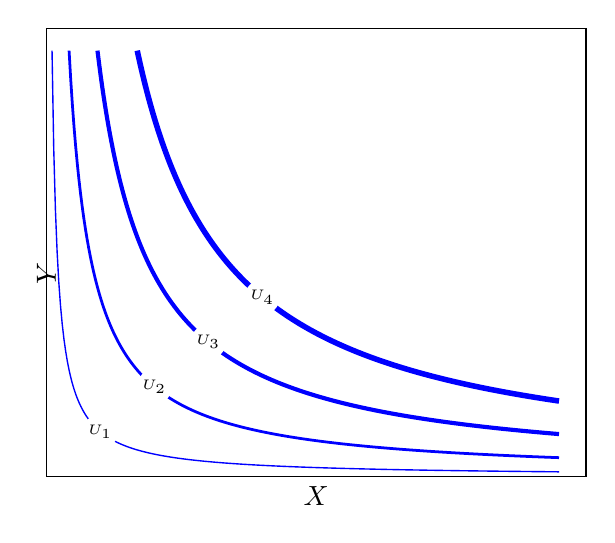
\begin{tikzpicture}
\begin{axis}[
	domain=0:10,
	xmin=0,xmax=10,ymin=0,ymax=10,
	xtick=\empty,	ytick=\empty,
	xticklabel=\ ,	yticklabel=\ ,
	xlabel style={below},xlabel=$X$,
	ylabel style={left},ylabel=$Y$,
	samples=300]
\addplot[draw=blue,line width=0.5pt,domain=1/9.5:9.5] {1/x};
\addplot[draw=blue,line width=1pt,domain=4/9.5:9.5] {4/x};
\addplot[draw=blue,line width=1.5pt,domain=9/9.5:9.5] {9/x};
\addplot[draw=blue,line width=2pt,domain=16/9.5:9.5] {16/x};
\node[fill=white,circle,inner sep=1pt,font=\tiny] at (axis cs:1,1) {$U_1$};
\node[fill=white,circle,inner sep=1pt,font=\tiny] at (axis cs:2,2) {$U_2$};
\node[fill=white,circle,inner sep=1pt,font=\tiny] at (axis cs:3,3) {$U_3$};
\node[fill=white,circle,inner sep=1pt,font=\tiny] at (axis cs:4,4) {$U_4$};
\end{axis}
\end{tikzpicture}
\caption{$U(x,y) = x^{1/2} y^{1/2}$}
\label{fig:indefferent-curves_c-daa}%
\end{subfigure}%
\begin{subfigure}[b]{0.5\textwidth}
\centering
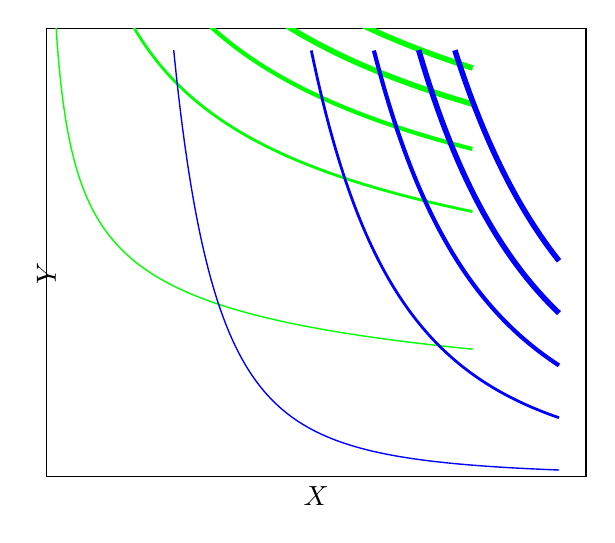
\begin{tikzpicture}
\begin{axis}[
	domain=0:10,
	xmin=0,xmax=10,ymin=0,ymax=10,
	xtick=\empty,	ytick=\empty,
	xticklabel=\ ,	yticklabel=\ ,
	xlabel style={below},xlabel=$X$,
	ylabel style={left},ylabel=$Y$,
	samples=300]
%反函数 cm={0,1,1,0,(0,0)}, tikz page 253 /tikz/cm={hai,hbi,hci,hdi,hcoordinatei}
\addplot[cm={0,1,1,0,(0,0)},draw=green,line width=0.5pt,domain=2.36:9.5] {125/(x^3)};
\addplot[cm={0,1,1,0,(0,0)},draw=green,line width=1pt,domain=4.91:9.5] {1125/(x^3)};
\addplot[cm={0,1,1,0,(0,0)},draw=green,line width=1.5pt,domain=6.07:9.5] {2125/(x^3)};
\addplot[cm={0,1,1,0,(0,0)},draw=green,line width=2pt,domain=6.90:9.5] {3125/(x^3)};
\addplot[cm={0,1,1,0,(0,0)},draw=green,line width=2pt,domain=7.57:9.5] {4125/(x^3)};
\addplot[draw=blue,line width=0.5pt,domain=2.36:9.5] {125/(x^3)};
\addplot[draw=blue,line width=1pt,domain=4.91:9.5] {1125/(x^3)};
\addplot[draw=blue,line width=1.5pt,domain=6.07:9.5] {2125/(x^3)};
\addplot[draw=blue,line width=2pt,domain=6.90:9.5] {3125/(x^3)};
\addplot[draw=blue,line width=2pt,domain=7.57:9.5] {4125/(x^3)};
\end{axis}
\end{tikzpicture}
\caption{\textcolor{blue}{$U(x,y) = x^{3/4} y^{1/4}$} 与 \textcolor{green}{$U(x,y) = x^{1/4} y^{3/4}$}}
\label{fig:indefferent-curves_c-dab}%
\end{subfigure}
\caption{柯布—道格拉斯函数的无差异曲线}
\label{fig:indefferent-curves_c-d}%%
}}
\end{figure}

\subsection[CES]{CES 效用函数}
\index{utility function 效用函数!CES 固定弹性替代}

CES 效用函数,也称作固定弹性替代效用函数(Constant Elasticity of Substitution),形如:

\begin{equation}
u=f(x,y)=\left[\alpha x^\rho +(1-\alpha)y^\rho\right]^{1/\rho}
\label{eq:ces-utility-function}
\end{equation}
其中$\alpha\in(0,1)$,$\rho\leq 1$,Cobb-Douglas 效用函数是 CES 效用函数在$\rho \to 0$时的特殊情况。

商品$x$的边际效用函数为,

\[MU_X=\alpha \left[\alpha x^\rho +(1-\alpha)y^\rho\right]^{\frac{1}{\rho}-1} x^{\rho-1}\]

商品$y$的边际效用函数为,

\[MU_Y=(1-\alpha)\left[\alpha x^\rho +(1-\alpha)y^\rho\right]^{\frac{1}{\rho}-1} y^{\rho-1}\]

\[\frac{dx}{dy}=-\frac{1-\alpha}{\alpha}\left(\frac{x}{y}\right)^{1-\rho}\]


\section*{推荐阅读}
\markright{推荐阅读}
\addcontentsline{toc}{section}{\hspace{-2.5em}推荐阅读}



\newpage
\section*{本章附录}
\markright{本章附录}
\addcontentsline{toc}{section}{\hspace{-2.5em}本章附录}
\label{sec:appendix-utility}

\subsection*{偏导数}